\section{Secondary wavetable results}
\label{app:secondary-results}

Moved from the main Results section to shorten the conference-length reading path.
Primary holdout, meta-compare, and converge claims remain in Section~\ref{sec:results}.

\paragraph{Superseded whole-curve freezes.}
Whole-curve prolonged-$R$ freezes ($R{\approx}0.991$ vs DualCosine ${\approx}0.825$) are not current results.
Selection and published comparison under v10.1 use $R_{\mathrm{blend}}{+}J$ with Noise2Noise as the primary neural baseline.

\subsection{Which families stay hard}
\label{sec:family-hardness}
On the fitted DenoiseOpt $100{,}000$-cycle bench, denoise score $D$ is lowest for \texttt{nonlinear} ($D\approx 0.39$) and \texttt{combo} ($D\approx 0.40$), then \texttt{triple\_mix} / \texttt{extreme\_overlay} ($D\approx 0.51$--$0.52$), while \texttt{harmonic\_fft} and \texttt{am\_fm} sit near $D\approx 0.69$--$0.70$.
Lit-combo champion family stress (prolonged residual) similarly ranks \texttt{open\_wrap\_bias} ($R\approx 0.83$) and \texttt{extreme\_overlay} / \texttt{combo} ($R\approx 0.88$--$0.89$) below \texttt{harmonic\_fft} ($R\approx 0.95$).
Hard sounds recur.

\paragraph{Superseded $5$k-gate freeze.}
At the reported $5$k-gate search freeze ($\approx 6{,}922$ clean iterations, $\approx 7.9$\,h on RTX~3090) the champion residual was $R\approx 0.99093$ with DualCosine $\approx 0.81658$ on the CUDA search runner ($\Delta R\approx{+}0.174$).
That freeze optimized whole-curve prolonged $R$.
It is superseded by $R_{\mathrm{blend}}$ for v10.1 selection.
Monitoring plots below come from that older freeze and should be read as search-trace artifacts, not as locked-protocol scores.

\subsection{Inference latency at matched score}
\label{sec:inference-latency}
Across the prior high-prolonged-$R$ fitted operators, we re-timed CUDA forward passes under locked $R_{\mathrm{blend}}$ (batch 64).
Live $R_{\mathrm{blend}}$ spreads more than the old prolonged band: the max-$R_{\mathrm{blend}}$ model is
\texttt{champion\_iter\_000265} ($R_{\mathrm{blend}}{\approx}0.9769$, $\approx 6.53$\,ms/batch, $\approx 94$k params).
The compact historically favorite \texttt{iter\_000235} remains lowest-latency among the top-5 distinct topologies
($R_{\mathrm{blend}}{\approx}0.9749$, $\approx 3.42$\,ms/batch, $\approx 37$k params).
Selection rule: maximize live $R_{\mathrm{blend}}$, then minimize latency inside $R\ge R_{\max}-5\cdot10^{-4}$.

\subsection{Top-5 architectures}
\label{sec:top5-arch}
Table~\ref{tab:top5} ranks five distinct fitted bake graphs from the CUDA inference bench
(\href{https://github.com/reeldemo/denoise-opt-meta/blob/master/paper/Unsupervised_Wrap-Discontinuity_Repair_in_Wavetable_Synthesis_via_Hybrid_GA-PPO_Meta-Search_v12/figures/inference_bench.json}{inference data}, batch 64), preferring live $R_{\mathrm{blend}}$ first and latency on ties,
and skipping near-duplicate copies of the same topology signature.

\begin{table}[htbp]
  \centering
  \caption{Top-5 distinct fitted architectures on the CUDA inference bench (batch 64) under $R_{\mathrm{blend}}$ ($\alpha{=}0.7$).
  $R_{\mathrm{saved}}$ is the checkpoint hint (often prolonged $R$); $R_{\mathrm{live}}$ is measured $R_{\mathrm{blend}}$.
  *Max-$R_{\mathrm{blend}}$ (also sole member of the $R\ge R_{\max}-5\cdot10^{-4}$ band here).}
  \label{tab:top5}
  \setlength{\tabcolsep}{3pt}
  \begin{adjustbox}{max width=\columnwidth}
\begin{tabular}{@{}lrrrr@{}}
    \toprule
    Tag & $R_{\mathrm{saved}}$ & $R_{\mathrm{live}}$ & ms/batch & params \\
    \midrule
    \texttt{iter\_000265}* & 0.9906 & 0.9769 & 6.53 & 93\,566 \\
    \texttt{iter\_000140} & 0.9906 & 0.9762 & 7.16 & 104\,484 \\
    \texttt{iter\_000133} & 0.9908 & 0.9752 & 7.16 & 104\,484 \\
    \texttt{iter\_000229} & 0.9909 & 0.9751 & 7.56 & 100\,500 \\
    \texttt{iter\_000235} & 0.9910 & 0.9749 & 3.42 & 37\,489 \\
    \bottomrule
  \end{tabular}
\end{adjustbox}\\[0.4em]
  {\footnotesize *Favorite under maximize-$R_{\mathrm{blend}}$ then latency. Compact \texttt{iter\_000235} is still the latency floor in this top-5.}
\end{table}

\label{sec:classical-vs-favorite}
Table~\ref{tab:canonical-methods} scores the classical (non-AI) bake set (no-bake, DualCosine, and \texttt{seam\_fir3}) plus the locked v10.1 hybrid favorite on the frozen corpus of Section~\ref{sec:dataset} (CUDA, batch 64, seed \texttt{20260719}) under $R_{\mathrm{blend}}$.
DualCosine reaches $R_{\mathrm{blend}}\approx 0.541$ ($\approx 1.66$\,ms/batch).
Active classical \texttt{seam\_fir3} reaches $0.884$ / $\approx 1.11$\,ms/batch ($0.888\pm0.009$ over five seeds).
No-bake (passthrough) scores $0.914$ ($0.917\pm0.009$).
The hybrid favorite reaches $0.970$ ($0.971\pm0.001$ over five seeds) at $\approx 5.99$\,ms/batch:
$\Delta R_{\mathrm{blend}} \approx {+}0.056$ vs no-bake and $\approx {+}0.429$ vs DualCosine.
Noise2Noise on the multi-family matrix is Appendix Table~\ref{tab:sota-main}. The four-board gate is Table~\ref{tab:n2n-vs-ours}.

\begin{table}[htbp]
  \centering
  \caption{Canonical holdout under $R_{\mathrm{blend}}$ ($\alpha{=}0.7$; seed \texttt{20260719}). Mean$\pm$std over five seeds. No-bake $=$ unrepaired engine. Favorite $=$ locked v10.1 hybrid champ.}
  \label{tab:canonical-methods}
  \setlength{\tabcolsep}{6pt}
  \begin{adjustbox}{max width=\columnwidth}
\begin{tabular}{@{}lrrr@{}}
    \toprule
    Method & $R_{\mathrm{blend}}$ & $R_{\mathrm{blend}}$ (5-seed) & ms/batch \\
    \midrule
    neural favorite & 0.9697 & $0.9708\pm0.0012$ & 5.99 \\
    no-bake (passthrough) & 0.9142 & $0.9166\pm0.0090$ & 1.06 \\
    \texttt{seam\_fir3} & 0.8842 & $0.8879\pm0.0087$ & 1.11 \\
    classic quadratic & 0.5742 & $0.5727\pm0.0318$ & 2.07 \\
    DualCosine & 0.5409 & $0.5420\pm0.0342$ & 1.66 \\
    cosine fade & 0.5409 & $0.5420\pm0.0342$ & 1.87 \\
    crossfade & 0.5310 & $0.5273\pm0.0311$ & 1.86 \\
    hann blend & 0.5197 & $0.5214\pm0.0337$ & 1.05 \\
    soft wide fade & 0.4828 & $0.4803\pm0.0258$ & 2.85 \\
    detrend & 0.3437 & $0.3453\pm0.0399$ & 0.96 \\
    ensemble detrend{+}DC{+}FIR & 0.3126 & $0.3100\pm0.0421$ & 2.00 \\
    \bottomrule
  \end{tabular}
\end{adjustbox}
\end{table}



\subsection{Multi-family comparison}
\label{sec:sota-main}

Does the locked hybrid favorite beat the classical non-AI board (no-bake, DualCosine, FIR, fades),
fixed MLP/CNN baselines, \emph{and} Noise2Noise across twenty generative families under $R_{\mathrm{blend}}$?
Appendix Table~\ref{tab:sota-main} reports mean$\pm$std over the 20-waveform multi-family set (Section~\ref{sec:dataset}) from the \href{https://github.com/reeldemo/denoise-opt-meta/blob/master/paper/Unsupervised_Wrap-Discontinuity_Repair_in_Wavetable_Synthesis_via_Hybrid_GA-PPO_Meta-Search_v12/figures/sota_matrix.json}{SOTA matrix}.
Appendix Figures~\ref{fig:sota-heatmap}--\ref{fig:sota-method-bars} plot the same ranking.
Primary reading is absolute $R_{\mathrm{blend}}$ rank:
Ours $0.934$, corrupt$\to$corrupt N2N $0.931$, seq CNN $0.920$, no-bake $0.893$,
\texttt{seam\_fir3} $0.868$, DualCosine $0.514$
(aligned with Table~\ref{tab:n2n-vs-ours} multifamily).
Fixed MLP-on-$R$ and CNN/U-Net-lite-on-$R$ (no outer NAS) sit between DualCosine and the neural rows.
Paired Wilcoxon signed-rank (normal approx.) of favorite vs DualCosine on the 20 waveforms: $W{=}0$, $p{\approx}8.9{\times}10^{-5}$, mean $\Delta R_{\mathrm{blend}}{=}{+}0.417$ (bootstrap 95\% CI $[0.398,0.435]$).
Vs no-bake the multifamily mean gap is $\approx{+}0.038$.
Vs corrupt$\to$corrupt N2N the mean-of-means gap is $\approx{+}0.003$ (mean win fraction $0.47$ across five seeds).

\paragraph{Cliff stratification (full).}
Main-text summary: Section~\ref{sec:cliff-strata}.
Appendix Table~\ref{tab:cliff-strata} stratifies the $4{,}096$-tile holdout by wrap-jump percentiles.

\subsection{Noise2Noise and sequence baselines}
\label{sec:n2n-baselines}

How does DenoiseOpt compare to true Noise2Noise-style and lightweight seq restorers on the same generator under $R_{\mathrm{blend}}$?
Primary corrupt$\to$corrupt N2N (train seed \texttt{424242}) reaches holdout $R_{\mathrm{blend}}\approx 0.975$ (Table~\ref{tab:n2n-vs-ours}), above the hybrid favorite ($0.970$).
On the $4{,}096$-tile cliff draw, sibling-supervised N2N reaches $0.981$ and seq LSTM $0.986$ (Appendix Table~\ref{tab:cliff-strata}).
Holdout tiles never enter training.
Classical DualCosine / \texttt{seam\_fir3} remain in Appendix Table~\ref{tab:cliff-strata}.
Figure~\ref{fig:n2n-vs-ours} plots the four-board $R_{\mathrm{blend}}$ comparison.

\begin{figure}[t]
  \centering
  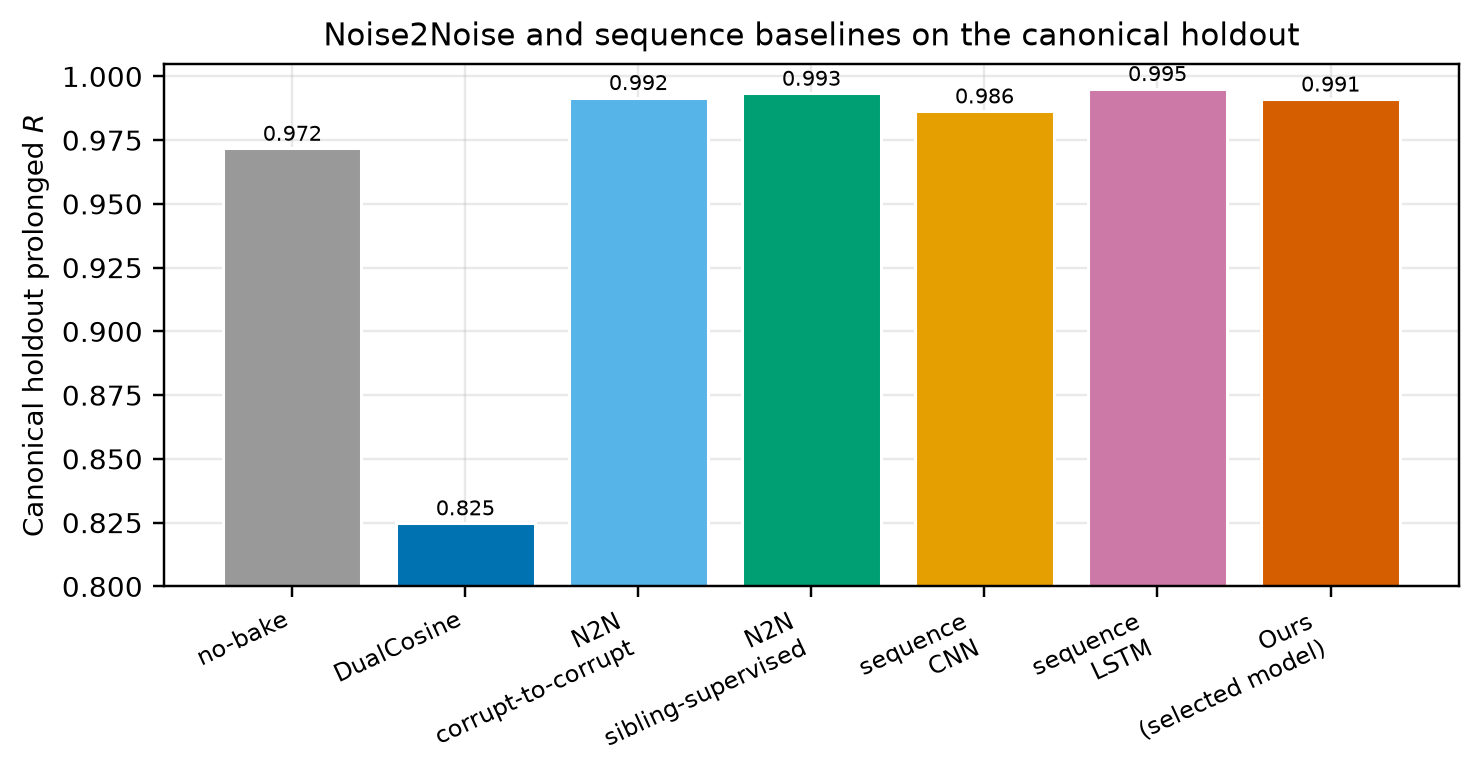
\includegraphics[width=\columnwidth]{figures/fig_n2n_vs_ours_bars.png}
  \caption{Canonical holdout $R_{\mathrm{blend}}$: N2N and seq baselines vs Ours (locked hybrid).
    Train seeds \texttt{424242}/\texttt{424243} are disjoint from holdout \texttt{20260719}.}
  \label{fig:n2n-vs-ours}
\end{figure}



\subsection{Factory exports and AKWF cycles}
\label{sec:real-wt}

Does the wrap protocol transfer beyond synthetic sine cliffs onto true exports and third-party OA cycles?
Table~\ref{tab:real-wt} scores ReelSynth-exported factory periods (primary realism) and Adventure Kid Waveforms (AKWF) CC0 single-cycle WAVs (secondary) after close-seam idealization and the same open-wrap cliff, under $R_{\mathrm{blend}}$.
Procedural stand-ins are demoted to tertiary smoke and no longer carry the primary realism claim.
On exported factory periods the favorite ($R_{\mathrm{blend}}{\approx}0.699$) trails no-bake / FIR / poly / N2N while still beating Dual Cosine ($0.589$).
On AKWF OA cycles the favorite ($0.679$) trails no-bake / N2N and beats Dual Cosine ($0.424$).
Export gaps are listed in Section~\ref{sec:limitations}.

\begin{table}[t]
  \centering
  \caption{Wavetable-native wrap protocol under $R_{\mathrm{blend}}$ ($\alpha{=}0.7$). Close-seam ideal $\to$ open-wrap cliff (seed \texttt{20260719}). Primary = ReelSynth export. Secondary = AKWF CC0 files.}
  \label{tab:real-wt}
  \setlength{\tabcolsep}{6pt}
  \begin{adjustbox}{max width=\columnwidth}
\begin{tabular}{@{}lrr@{}}
    \toprule
    Method & Export & AKWF OA \\
    \midrule
    \texttt{seam\_fir3} & 0.863 & 0.725 \\
    poly seam ($d{=}3$) & 0.846 & 0.696 \\
    no-bake & 0.845 & 0.702 \\
    endpoint-pin (mean) & 0.792 & 0.745 \\
    N2N corrupt$\to$corrupt & 0.771 & 0.731 \\
    seq CNN1D & 0.706 & 0.677 \\
    neural favorite & 0.699 & 0.679 \\
    DualCosine & 0.589 & 0.424 \\
    seq LSTM & 0.628 & 0.579 \\
    \bottomrule
  \end{tabular}
\end{adjustbox}
\end{table}

\subsection{Polynomial baseline and endpoint pinning}
\label{sec:poly-jump}

Does a cheap classical poly fitter close the residual, and does endpoint pinning show the wrap-jump vs $R_{\mathrm{blend}}$ tradeoff?
A seam-local degree-3 polynomial fitter (no learning) reaches canonical $R_{\mathrm{blend}}\approx 0.917$ (slightly above no-bake $0.914$) with wrap-jump essentially unchanged (\href{https://github.com/reeldemo/denoise-opt-meta/blob/master/paper/Unsupervised_Wrap-Discontinuity_Repair_in_Wavetable_Synthesis_via_Hybrid_GA-PPO_Meta-Search_v12/figures/poly_baseline.json}{polynomial results}).
SSM seq models are deferred. The LSTM remains the supervised seq ceiling.
An endpoint-pin control (\href{https://github.com/reeldemo/denoise-opt-meta/blob/master/paper/Unsupervised_Wrap-Discontinuity_Repair_in_Wavetable_Synthesis_via_Hybrid_GA-PPO_Meta-Search_v12/figures/jump_control.json}{pinning results}) drives wrap-jump to $0$ on all / hard subsets while dropping $R_{\mathrm{blend}}$ (all $0.733$, hard $0.597$).
Methods that zero wrap-jump are not the same objective as $R_{\mathrm{blend}}$ (Limitations).

\subsection{Classical virtual-analog seam repairs}
\label{sec:va-seam-baselines}

Do the cited VA antialias tools~\cite{stilson1996,nam2009polyblep,esqueda2016blamp} beat DualCosine on $R_{\mathrm{blend}}$ when applied as cycle-local seam residuals?

\paragraph{What each operator changes.}
Figure~\ref{fig:va-seam-techniques} shows the family on one high-wrap sine{+}cliff tile (same seed and tile as Figure~\ref{fig:intro-sine}).
\textbf{BLIT/BLEP} (Stilson/Smith lineage) treats the wrap as a value step.
It subtracts a band-limited step residual (here a raised-cosine BLEP-family lobe scaled by the measured wrap jump) so the tiled click spectrum is softened near the seam.
\textbf{PolyBLEP} (Nam et al.) is a cheap polynomial surrogate of that step residual with fractional-delay support near phase wrap.
It edits only a few samples on each side of the discontinuity.
\textbf{BLAMP} (Esqueda et al.) corrects a slope or corner jump (discontinuity in the first derivative), which matters for triangles, rectification, and hard clipping.
On a pure value cliff the slope jump is small, so BLAMP is nearly a no-bake passthrough.
\textbf{DualCosine} (our classical bake baseline) fades both ends of the stored period with raised-cosine windows.
It does not insert a BLEP-style residual.
It trades wrap energy for a wide end-fade distortion that $R_{\mathrm{blend}}$ penalizes on hard cliffs.

\paragraph{Scores.}
Table~\ref{tab:va-seam-blep} reports batch means from the \href{https://github.com/reeldemo/denoise-opt-meta/blob/master/paper/Unsupervised_Wrap-Discontinuity_Repair_in_Wavetable_Synthesis_via_Hybrid_GA-PPO_Meta-Search_v12/figures/va_seam_blep.json}{VA results} (seed \texttt{20260719}, batch 64) under $R_{\mathrm{blend}}$.
Code is in the \href{https://github.com/reeldemo/reelsynth}{ReelSynth repository}: PolyBLEP matches \texttt{osc::va::poly\_blep}, BLIT/BLEP uses a raised-cosine step residual, and BLAMP applies a polyBLAMP lobe to the wrap slope jump.
PolyBLEP reaches mean $R_{\mathrm{blend}}\approx 0.795$ ($\Delta\approx{+}0.254$ vs DualCosine) but trails no-bake / \texttt{seam\_fir3}.
BLIT/BLEP nearly zeros wrap-jump ($0.004$), yet mean $R_{\mathrm{blend}}$ falls to $0.632$ and hard cliffs collapse to $0.351$.
BLAMP stays near no-bake on this value-cliff geometry (mean $0.914$).
On the annotated severe tile in Figure~\ref{fig:va-seam-techniques}, tile $R_{\mathrm{blend}}$ is lower still (PolyBLEP $\approx 0.726$, BLIT/BLEP $\approx 0.385$, Dual Cosine $0.300$, BLAMP $\approx$ engine).
We score these classical tools, not only cite them: they beat DualCosine on mean $R_{\mathrm{blend}}$ in places, and none matches the locked hybrid favorite on holdout $R_{\mathrm{blend}}$.

\begin{figure}[t]
  \centering
  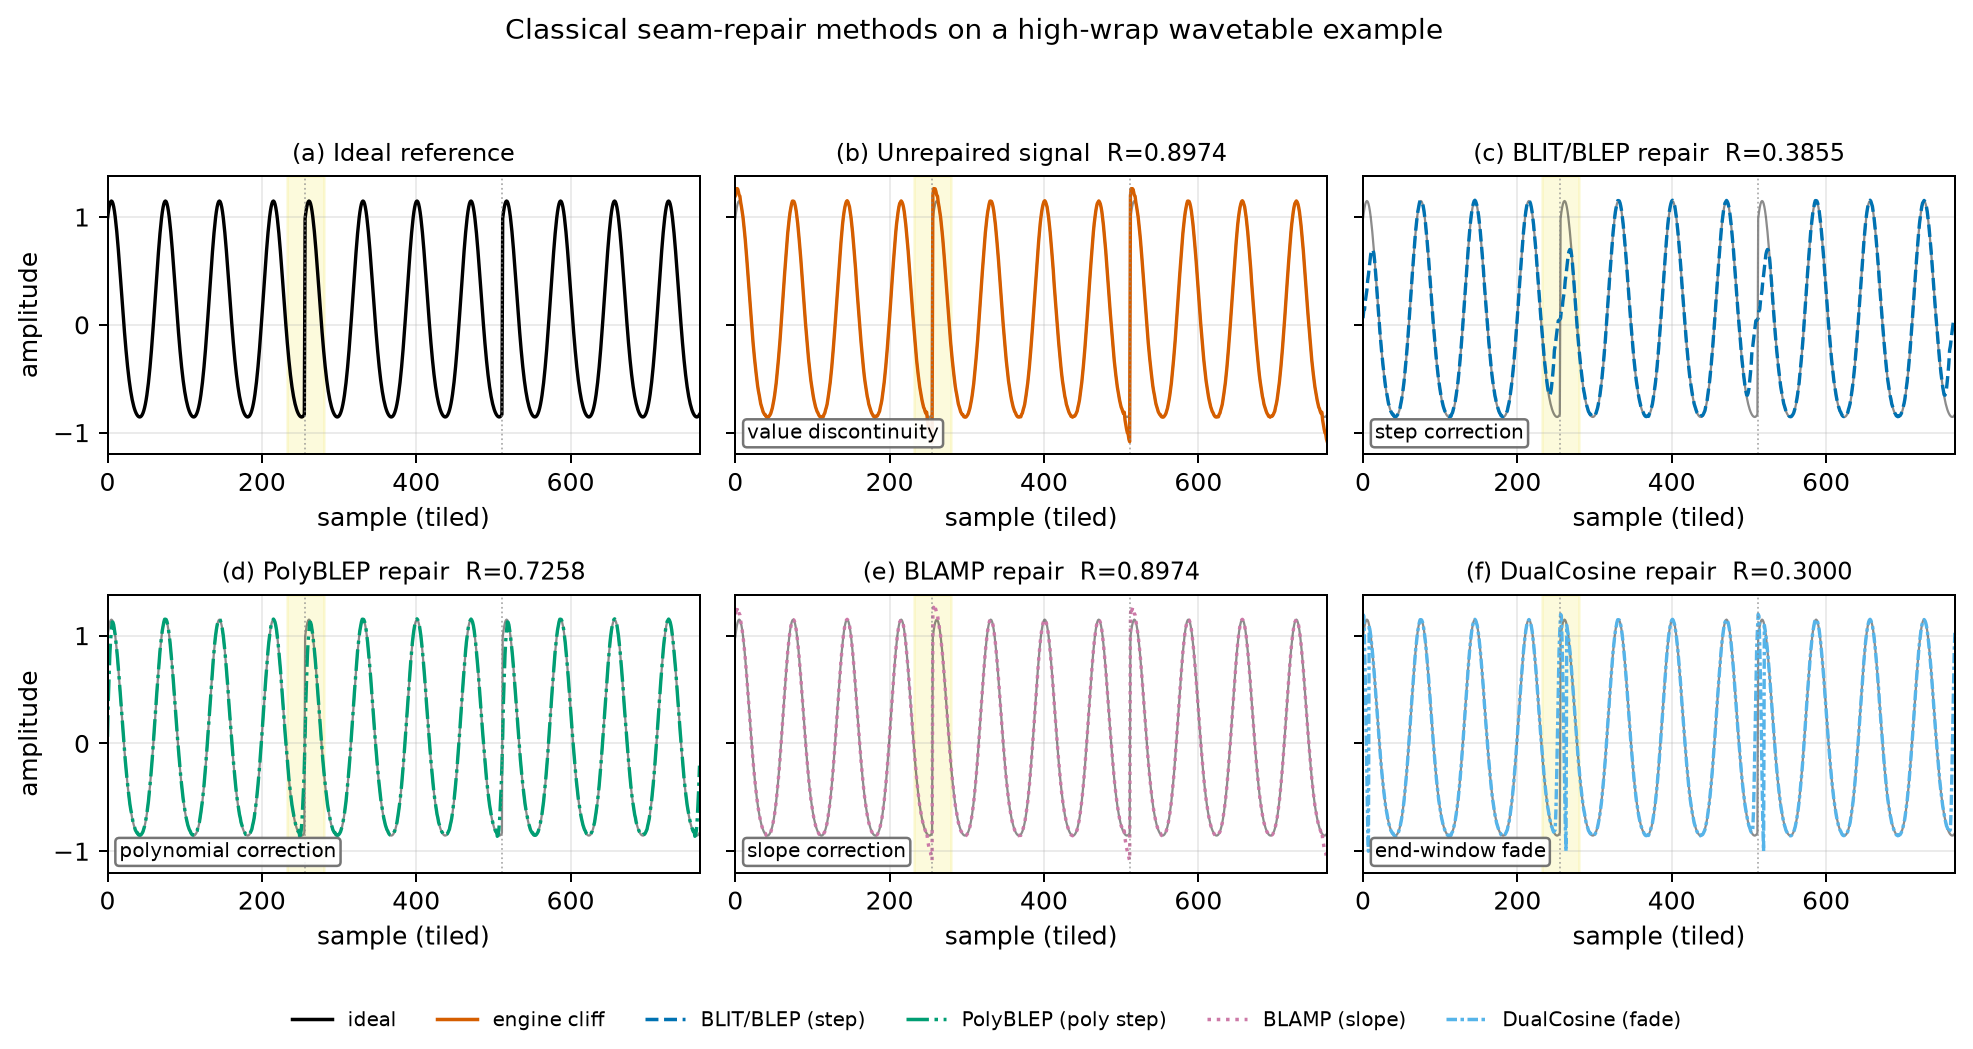
\includegraphics[width=\columnwidth]{figures/fig_va_seam_techniques.png}
  \caption{Classical VA seam techniques on one cracked sine{+}cliff tile
  (seed~\texttt{20260719}, tile~46).
  (a)~ideal; (b)~cracked engine; (c)~BLIT/BLEP; (d)~PolyBLEP; (e)~BLAMP; (f)~DualCosine.
  Batch means: Table~\ref{tab:va-seam-blep}.}
  \label{fig:va-seam-techniques}
\end{figure}

\begin{table}[t]
  \centering
  \caption{Classical VA seam repairs under $R_{\mathrm{blend}}$ ($\alpha{=}0.7$; seed \texttt{20260719}).
  Holdout $R_{\mathrm{blend}}$, seam-local edge RMSE, cliff top-10\% $R_{\mathrm{blend}}$, multi-family mean.}
  \label{tab:va-seam-blep}
  \setlength{\tabcolsep}{3pt}
  \footnotesize
  \begin{tabular}{@{}lcccc@{}}
    \toprule
    Method & $R$ & edge & top10 & multi \\
    \midrule
    BLAMP & 0.914 & 0.080 & 0.922 & 0.893 \\
    no-bake & 0.914 & 0.080 & 0.922 & 0.893 \\
    \texttt{seam\_fir3} & 0.884 & 0.112 & 0.869 & 0.868 \\
    PolyBLEP & 0.795 & 0.205 & 0.690 & 0.784 \\
    BLIT/BLEP & 0.632 & 0.365 & 0.351 & 0.612 \\
    DualCosine & 0.541 & 0.506 & 0.305 & 0.514 \\
    \bottomrule
  \end{tabular}\\[0.35em]
  {\footnotesize Latency (CUDA): PolyBLEP ${\approx}0.87$\,ms/batch, DualCosine ${\approx}1.46$, BLIT/BLEP ${\approx}71$, BLAMP ${\approx}20$.}
\end{table}





\subsection{When search helps vs classical methods}
\label{sec:transfer}

Per-cycle $\Delta R$ on export, AKWF, Rust \texttt{sound\_bench}, and sine{+}cliff holdout
(\href{https://github.com/reeldemo/denoise-opt-meta/blob/master/paper/Unsupervised_Wrap-Discontinuity_Repair_in_Wavetable_Synthesis_via_Hybrid_GA-PPO_Meta-Search_v12/figures/transfer_failures.json}{transfer results}):
favorite win-rate vs Dual Cosine is high on sine cliffs ($1.00$) and AKWF ($0.88$), and moderate on export ($0.64$) / Rust ($0.75$).
Win-rate vs no-bake is high only on sine cliffs ($0.92$) and collapses on export ($0.24$) / Rust ($0.20$).
Search value is highest on hard cliffs and when compact bake graphs are needed without engine$\to$ideal labels at search time.
Export / Rust gaps vs no-bake are listed in Section~\ref{sec:limitations}.

\subsection{Transfer to Rust engine tiles}
\label{sec:rust-bench}

Table~\ref{tab:rust-bench} scores the Python-trained favorite on 20 Rust-exported tiles under $R_{\mathrm{blend}}$.
The favorite beats Dual Cosine on mean $\Delta R_{\mathrm{blend}}{+}0.082$, but the signed-rank test is not significant at $\alpha{=}0.05$ ($p{\approx}0.30$),
and absolute score trails no-bake and \texttt{seam\_fir3}.
The primary SOTA claim remains the Python multi-family matrix.

\begin{table}[t]
  \centering
  \caption{Rust \texttt{sound\_bench} transfer ($n{=}20$) under $R_{\mathrm{blend}}$ ($\alpha{=}0.7$).
  $\Delta$ is vs Dual Cosine.}
  \label{tab:rust-bench}
  \setlength{\tabcolsep}{6pt}
  \begin{adjustbox}{max width=\columnwidth}
\begin{tabular}{@{}lrr@{}}
    \toprule
    Method & $R_{\mathrm{blend}}$ & $\Delta$ vs DC \\
    \midrule
    no-bake & $0.846\pm0.171$ & ${+}0.422$ \\
    \texttt{seam\_fir3} & $0.751\pm0.157$ & ${+}0.327$ \\
    neural favorite & $0.506\pm0.236$ & ${+}0.082$ \\
    classic quadratic & $0.474\pm0.186$ & ${+}0.050$ \\
    Dual Cosine / cosine fade & $0.424\pm0.187$ & $0$ \\
    \bottomrule
  \end{tabular}
\end{adjustbox}
\end{table}
